\section{Semantic Interpretation of the Clusters}
\label{sec:experiments_semantic_interpretation_of_the_clusters}

The metrics reported in Section~\ref{sec:experiments_clustering_quality_of_the_latent_space} evaluate the \gls{ls} clusterings quantitatively but do not indicate what the resulting clusters actually represent.
This section complements them with a qualitative, hand-labeled inspection of the clusters obtained for each environment.

For each environment, two clusterings are selected for the qualitative analysis.
They are obtained using two different numbers of clusters and may correspond to different layers of the network.
The choice of the layer and the number of clusters is based on the following criteria:
\begin{itemize}
\item \textbf{High \gls{acu}:} The selected clustering should achieve a sufficiently high \gls{acu}, indicating a good balance between consistency and abstraction.
\item \textbf{Manual analysis:} The number of clusters must remain small enough to allow the resulting clusters to be examined manually.
\item \textbf{Limited use of two-cluster partitions:} Clusterings with two clusters often achieve a high \gls{acu}, but provide limited information about the organization of the \gls{ls}. Therefore, at most one of the two selected clusterings uses two clusters, while the other uses a larger number of clusters to provide a more detailed view of the \gls{ls}.
\end{itemize}

Only these two clusterings are discussed below, but the clusters obtained for every analyzed layer can also be inspected.\footnote{Images of the clusters obtained for every analyzed layer have been archived on Zenodo \LinkClusterImages.}

\newcommand{\qualitativeClusterImageScale}{0.20}

\newlength{\qualitativeClusterImageWidth}
\settowidth{\qualitativeClusterImageWidth}{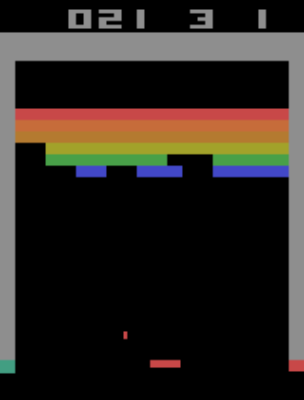
\includegraphics[scale=\qualitativeClusterImageScale]{figures/experiments/pictures/breakout/qualitative/cluster_0/image_1.png}}

% Spacing between the two screenshots of a same cluster.
\newlength{\qualitativeClusterImageGap}
\setlength{\qualitativeClusterImageGap}{0.1cm}

% Spacing between two clusters on the same row of a figure.
\newlength{\qualitativeClusterGap}
\setlength{\qualitativeClusterGap}{0.4cm}

% Vertical spacing between two rows of clusters in a same figure.
\newlength{\qualitativeClusterRowGap}
\setlength{\qualitativeClusterRowGap}{0.3cm}

% The gap is inserted before every cluster except the first one of a figure, so that
% no row carries a trailing gap and every row is centered on the same axis.
\newif\ifqualitativeFirstCluster

% Start of every cluster figure: centers the clusters and applies the row spacing.
\newcommand{\qualitativeClusterFigureSetup}{%
    \centering
    \setlength{\lineskiplimit}{1000pt}%
    \setlength{\lineskip}{\qualitativeClusterRowGap}%
    \qualitativeFirstClustertrue
}

% A cluster shown with two example screenshots, always kept on the same line, labeled with a letter.
\newcommand{\qualitativeClusterTwo}[3]{%
    \ifqualitativeFirstCluster\qualitativeFirstClusterfalse\else\hspace{\qualitativeClusterGap}\fi
    \begin{minipage}[t]{\dimexpr 2\qualitativeClusterImageWidth+\qualitativeClusterImageGap\relax}
        \centering
        \includegraphics[scale=\qualitativeClusterImageScale]{#1}\hspace{\qualitativeClusterImageGap}\includegraphics[scale=\qualitativeClusterImageScale]{#2}\par
        \small\textbf{#3}
    \end{minipage}%
}

\EnableCompactFloats
\newpage
\subsection{\BreakoutName}

Two clusterings are examined for \BreakoutName (Table~\ref{tab:qualitative_breakout_metrics}), obtained at layer 4 with $K=2$ and at layer 6b with $K=5$.

At layer 4 (Figure~\ref{fig:qualitative_breakout_alt}), the partition captures the position of the ball relative to the brick wall.
The ball remains below the wall in cluster A.
The ball has passed behind the wall in cluster B, allowing it to continue clearing bricks without further interaction with the paddle.

At layer 6b (Figure~\ref{fig:qualitative_breakout}), the partition again isolates situations in which the ball has passed behind the wall in cluster E.
It also identifies the digging of a tunnel through the left side of the wall in cluster C.
Finally, it distinguishes different paddle positions at the beginning of the episode in clusters D, F, and G.

The clustering at layer 4 with $K=2$ is almost perfectly reproducible across surrogate policies, with a \gls{cu} of $0.99$ and an \gls{acu} of $0.87$.
The clustering at layer 6b with $K=5$ is less consistent, with a \gls{cu} of $0.79$ and an \gls{acu} of $0.61$, but reveals additional information about the organization of the \gls{ls}.

\vfill
\begin{table}[H]
    \centering
    \begin{tblr}{
        width=\linewidth,
        colspec={Q[c,wd=1.6cm] X[l]},
        cells = {valign=m},
        rowsep=2pt,
        hline{1,Z} = {1pt},
        hline{4} = {0.5pt},
        hline{2,5} = {0.3pt},
        row{1,4} = {bg=black!8, font=\bfseries},
        column{1} = {font=\bfseries}
    }
        \SetCell[c=2]{l} \makebox[1.9cm][l]{Layer 4}\makebox[1.4cm][l]{$K=2$}\makebox[2.75cm][l]{\gls{cu} 0.99}\makebox[2.75cm][l]{\gls{as} 0.88}\gls{acu} 0.87 & \\
        A & The ball is below the brick wall. \\
        B & The ball passes behind the brick wall. \\
        \SetCell[c=2]{l} \makebox[1.9cm][l]{Layer 6b}\makebox[1.4cm][l]{$K=5$}\makebox[2.75cm][l]{\gls{cu} 0.79}\makebox[2.75cm][l]{\gls{as} 0.82}\gls{acu} 0.61 & \\
        C & Digging a tunnel through the left side of the wall. \\
        D & Start of the episode, paddle on the right. \\
        E & The ball is behind the brick wall. \\
        F & Start of the episode, paddle in the middle. \\
        G & Start of the episode, paddle on the left. \\
    \end{tblr}
    \caption{\glsfmtshort{cu}, \glsfmtshort{as}, and \glsfmtshort{acu} of the two clusterings analyzed in the \BreakoutName environment.}
    \label{tab:qualitative_breakout_metrics}
\end{table}
\vfill

\newpage
\vspace*{\fill}
\begin{figure}[H]
    \qualitativeClusterFigureSetup
    \qualitativeClusterTwo
        {figures/experiments/pictures/breakout/qualitative_alt/cluster_0/image_1.png}
        {figures/experiments/pictures/breakout/qualitative_alt/cluster_0/image_2.png}
        {A}
    \qualitativeClusterTwo
        {figures/experiments/pictures/breakout/qualitative_alt/cluster_1/image_1.png}
        {figures/experiments/pictures/breakout/qualitative_alt/cluster_1/image_2.png}
        {B}
    \caption{Clusters A--B identified by \glsfmtshort{car} in the \BreakoutName environment (layer 4, $K=2$).}
    \label{fig:qualitative_breakout_alt}
\end{figure}


\begin{figure}[H]
    \qualitativeClusterFigureSetup
    \qualitativeClusterTwo
        {figures/experiments/pictures/breakout/qualitative/cluster_0/image_1.png}
        {figures/experiments/pictures/breakout/qualitative/cluster_0/image_2.png}
        {C}
    \qualitativeClusterTwo
        {figures/experiments/pictures/breakout/qualitative/cluster_1/image_1.png}
        {figures/experiments/pictures/breakout/qualitative/cluster_1/image_2.png}
        {D}
    \qualitativeClusterTwo
        {figures/experiments/pictures/breakout/qualitative/cluster_2/image_1.png}
        {figures/experiments/pictures/breakout/qualitative/cluster_2/image_2.png}
        {E}
    \qualitativeClusterTwo
        {figures/experiments/pictures/breakout/qualitative/cluster_3/image_1.png}
        {figures/experiments/pictures/breakout/qualitative/cluster_3/image_2.png}
        {F}
    \qualitativeClusterTwo
        {figures/experiments/pictures/breakout/qualitative/cluster_4/image_1.png}
        {figures/experiments/pictures/breakout/qualitative/cluster_4/image_2.png}
        {G}
    \caption{Clusters C--G identified by \glsfmtshort{car} in the \BreakoutName environment (layer 6b, $K=5$).}
    \label{fig:qualitative_breakout}
\end{figure}

\vfill

\cleartoleftpage
\subsection{\MarioBrosName}

Two clusterings are examined for \MarioBrosName (Table~\ref{tab:qualitative_mario_bros_metrics}), both obtained at layer 3, with $K=3$ and $K=5$.

With $K=3$ (Figure~\ref{fig:qualitative_mario_bros}), the partition is organized around the location of the action.
Mario fights enemies on the left side of the screen in cluster A.
He fights enemies on the right side of the screen in cluster C.
The POW block is present in cluster B, isolating a fixed and recognizable element of the level.

With $K=5$ (Figure~\ref{fig:qualitative_mario_bros_alt}), the partition provides a more detailed description of the situations occurring in the level.
Mario is on the top-left platform in cluster D.
Mario attacks enemies at the top left in cluster F.
Mario hits enemies from below in cluster H.
Mario simply moves through the level in cluster G.
The POW block remains isolated in cluster E.

Increasing $K$ from $3$ to $5$ lowers \gls{cu} from $0.84$ to $0.75$.
The \gls{as} remains nearly unchanged, with values of $0.66$ and $0.65$.
This results in a decrease in \gls{acu} from $0.50$ to $0.40$.

\vfill
\begin{table}[H]
    \centering
    \begin{tblr}{
        width=\linewidth,
        colspec={Q[c,wd=1.6cm] X[l]},
        cells = {valign=m},
        rowsep=2pt,
        hline{1,Z} = {1pt},
        hline{5} = {0.5pt},
        hline{2,6} = {0.3pt},
        row{1,5} = {bg=black!8, font=\bfseries},
        column{1} = {font=\bfseries}
    }
        \SetCell[c=2]{l} \makebox[1.9cm][l]{Layer 3}\makebox[1.4cm][l]{$K=3$}\makebox[2.75cm][l]{\gls{cu} 0.84}\makebox[2.75cm][l]{\gls{as} 0.66}\gls{acu} 0.50 & \\
        A & Mario fights enemies on the left side of the screen. \\
        B & The POW block is present. \\
        C & Mario fights enemies on the right side of the screen. \\
        \SetCell[c=2]{l} \makebox[1.9cm][l]{Layer 3}\makebox[1.4cm][l]{$K=5$}\makebox[2.75cm][l]{\gls{cu} 0.75}\makebox[2.75cm][l]{\gls{as} 0.65}\gls{acu} 0.40 & \\
        D & Mario is on the top-left platform. \\
        E & The POW block is present. \\
        F & Mario attacks the enemies at the top right. \\
        G & Mario moves through the level. \\
        H & Mario hits enemies from below on the left side. \\
    \end{tblr}
    \caption{\glsfmtshort{cu}, \glsfmtshort{as}, and \glsfmtshort{acu} of the two clusterings analyzed in the \MarioBrosName environment.}
    \label{tab:qualitative_mario_bros_metrics}
\end{table}
\vfill

\newpage
\vspace*{\fill}
\begin{figure}[H]
    \qualitativeClusterFigureSetup
    \qualitativeClusterTwo
        {figures/experiments/pictures/mario_bros/qualitative/cluster_0/image_1.png}
        {figures/experiments/pictures/mario_bros/qualitative/cluster_0/image_2.png}
        {A}
    \qualitativeClusterTwo
        {figures/experiments/pictures/mario_bros/qualitative/cluster_1/image_1.png}
        {figures/experiments/pictures/mario_bros/qualitative/cluster_1/image_2.png}
        {B}
    \qualitativeClusterTwo
        {figures/experiments/pictures/mario_bros/qualitative/cluster_2/image_1.png}
        {figures/experiments/pictures/mario_bros/qualitative/cluster_2/image_2.png}
        {C}
    \caption{Clusters A--C identified by \glsfmtshort{car} in the \MarioBrosName environment (layer 3, $K=3$).}
    \label{fig:qualitative_mario_bros}
\end{figure}


\begin{figure}[H]
    \qualitativeClusterFigureSetup
    \qualitativeClusterTwo
        {figures/experiments/pictures/mario_bros/qualitative_alt/cluster_0/image_1.png}
        {figures/experiments/pictures/mario_bros/qualitative_alt/cluster_0/image_2.png}
        {D}
    \qualitativeClusterTwo
        {figures/experiments/pictures/mario_bros/qualitative_alt/cluster_1/image_1.png}
        {figures/experiments/pictures/mario_bros/qualitative_alt/cluster_1/image_2.png}
        {E}
    \qualitativeClusterTwo
        {figures/experiments/pictures/mario_bros/qualitative_alt/cluster_2/image_1.png}
        {figures/experiments/pictures/mario_bros/qualitative_alt/cluster_2/image_2.png}
        {F}
    \qualitativeClusterTwo
        {figures/experiments/pictures/mario_bros/qualitative_alt/cluster_3/image_1.png}
        {figures/experiments/pictures/mario_bros/qualitative_alt/cluster_3/image_2.png}
        {G}
    \qualitativeClusterTwo
        {figures/experiments/pictures/mario_bros/qualitative_alt/cluster_4/image_1.png}
        {figures/experiments/pictures/mario_bros/qualitative_alt/cluster_4/image_2.png}
        {H}
    \caption{Clusters D--H identified by \glsfmtshort{car} in the \MarioBrosName environment (layer 3, $K=5$).}
    \label{fig:qualitative_mario_bros_alt}
\end{figure}

\vfill

\cleartoleftpage
\subsection{\MsPacManName}

Two clusterings are examined for \MsPacManName (Table~\ref{tab:qualitative_ms_pacman_metrics}), obtained at layer 6b with $K=3$ and at layer 4 with $K=5$.

With $K=3$ (Figure~\ref{fig:qualitative_ms_pacman}), the partition captures the progress and state of the game rather than a specific spatial feature of the observation.
The start of the episode is captured in cluster B.
The middle of the episode is captured in cluster A.
The end of the episode is captured in cluster C.

With $K=5$ (Figure~\ref{fig:qualitative_ms_pacman_alt}), the partition provides a more detailed description of the episode.
The initial animation, during which the character cannot move, is isolated in cluster H.
The beginning of actual play is captured in cluster F.
A situation specific to the game mechanics, in which Pac-Man is in booster mode and waits in front of the ghost spawn to eat the ghosts, is isolated in cluster D.
The end of the episode, when at most one power pellet remains, is separated into two similar clusters, E and G.

The two clusterings have the same \gls{cu} of $0.88$.
The clustering at layer 4 has a lower \gls{as} of $0.47$ compared with $0.52$ at layer 6b.
This results in a lower \gls{acu} of $0.35$ compared with $0.40$.

\vfill
\begin{table}[H]
    \centering
    \begin{tblr}{
        width=\linewidth,
        colspec={Q[c,wd=1.6cm] X[l]},
        cells = {valign=m},
        rowsep=2pt,
        hline{1,Z} = {1pt},
        hline{5} = {0.5pt},
        hline{2,6} = {0.3pt},
        row{1,5} = {bg=black!8, font=\bfseries},
        column{1} = {font=\bfseries}
    }
        \SetCell[c=2]{l} \makebox[1.9cm][l]{Layer 6b}\makebox[1.4cm][l]{$K=3$}\makebox[2.75cm][l]{\gls{cu} 0.88}\makebox[2.75cm][l]{\gls{as} 0.52}\gls{acu} 0.40 & \\
        A & Middle of the episode. \\
        B & Start of the episode. \\
        C & End of the episode. \\
        \SetCell[c=2]{l} \makebox[1.9cm][l]{Layer 4}\makebox[1.4cm][l]{$K=5$}\makebox[2.75cm][l]{\gls{cu} 0.88}\makebox[2.75cm][l]{\gls{as} 0.47}\gls{acu} 0.35 & \\
        D & Pac-Man is in booster mode and waits in front of the ghost spawn to eat the ghosts. \\
        E & End of the episode, at most one power pellet remains (similar to cluster G). \\
        F & Start of the episode. \\
        G & End of the episode, at most one power pellet remains (similar to cluster E). \\
        H & Start-of-episode animation, the character cannot move. \\
    \end{tblr}
    \caption{\glsfmtshort{cu}, \glsfmtshort{as}, and \glsfmtshort{acu} of the two clusterings analyzed in the \MsPacManName environment.}
    \label{tab:qualitative_ms_pacman_metrics}
\end{table}
\vfill

\newpage
\vspace*{\fill}
\begin{figure}[H]
    \qualitativeClusterFigureSetup
    \qualitativeClusterTwo
        {figures/experiments/pictures/ms_pacman/qualitative/cluster_0/image_1.png}
        {figures/experiments/pictures/ms_pacman/qualitative/cluster_0/image_2.png}
        {A}
    \qualitativeClusterTwo
        {figures/experiments/pictures/ms_pacman/qualitative/cluster_1/image_1.png}
        {figures/experiments/pictures/ms_pacman/qualitative/cluster_1/image_2.png}
        {B}
    \qualitativeClusterTwo
        {figures/experiments/pictures/ms_pacman/qualitative/cluster_2/image_1.png}
        {figures/experiments/pictures/ms_pacman/qualitative/cluster_2/image_2.png}
        {C}
    \caption{Clusters A--C identified by \glsfmtshort{car} in the \MsPacManName environment (layer 6b, $K=3$).}
    \label{fig:qualitative_ms_pacman}
\end{figure}


\begin{figure}[H]
    \qualitativeClusterFigureSetup
    \qualitativeClusterTwo
        {figures/experiments/pictures/ms_pacman/qualitative_alt/cluster_0/image_1.png}
        {figures/experiments/pictures/ms_pacman/qualitative_alt/cluster_0/image_2.png}
        {D}
    \qualitativeClusterTwo
        {figures/experiments/pictures/ms_pacman/qualitative_alt/cluster_1/image_1.png}
        {figures/experiments/pictures/ms_pacman/qualitative_alt/cluster_1/image_2.png}
        {E}
    \qualitativeClusterTwo
        {figures/experiments/pictures/ms_pacman/qualitative_alt/cluster_2/image_1.png}
        {figures/experiments/pictures/ms_pacman/qualitative_alt/cluster_2/image_2.png}
        {F}
    \qualitativeClusterTwo
        {figures/experiments/pictures/ms_pacman/qualitative_alt/cluster_3/image_1.png}
        {figures/experiments/pictures/ms_pacman/qualitative_alt/cluster_3/image_2.png}
        {G}
    \qualitativeClusterTwo
        {figures/experiments/pictures/ms_pacman/qualitative_alt/cluster_4/image_1.png}
        {figures/experiments/pictures/ms_pacman/qualitative_alt/cluster_4/image_2.png}
        {H}
    \caption{Clusters D--H identified by \glsfmtshort{car} in the \MsPacManName environment (layer 4, $K=5$).}
    \label{fig:qualitative_ms_pacman_alt}
\end{figure}

\vfill

\newpage
\subsection{\PongName}

Two clusterings are examined for \PongName (Table~\ref{tab:qualitative_pong_metrics}), obtained at layer 2 with $K=2$ and at layer 3 with $K=3$.

At layer 2 (Figure~\ref{fig:qualitative_pong_alt}), the partition separates the observations according to the number of digits in the player's score.
A one-digit score corresponds to cluster A.
A two-digit score corresponds to cluster B.
This reflects the progress of the game, but only through its visual display at the top of the screen.
The partition therefore captures a feature of the observation that provides no information about how the agent plays.

At layer 3 (Figure~\ref{fig:qualitative_pong}), the partition instead follows the vertical position of the ball.
The ball is at the top of the field in cluster C.
It is in the middle of the field in cluster D.
It is at the bottom of the field in cluster E.
This feature directly determines where the agent needs to place its paddle.

The clustering at layer 2 is perfectly reproducible and perfectly abstract, with \gls{cu}, \gls{as}, and \gls{acu} all equal to $1.00$.
The clustering at layer 3 is less consistent, with a \gls{cu} of $0.67$, and reaches a lower \gls{acu} of $0.65$.

\vfill
\begin{table}[H]
    \centering
    \begin{tblr}{
        width=\linewidth,
        colspec={Q[c,wd=1.6cm] X[l]},
        cells = {valign=m},
        rowsep=2pt,
        hline{1,Z} = {1pt},
        hline{4} = {0.5pt},
        hline{2,5} = {0.3pt},
        row{1,4} = {bg=black!8, font=\bfseries},
        column{1} = {font=\bfseries}
    }
        \SetCell[c=2]{l} \makebox[1.9cm][l]{Layer 2}\makebox[1.4cm][l]{$K=2$}\makebox[2.75cm][l]{\gls{cu} 1.00}\makebox[2.75cm][l]{\gls{as} 1.00}\gls{acu} 1.00 & \\
        A & The player's score has two digits. \\
        B & The player's score has one digit. \\
        \SetCell[c=2]{l} \makebox[1.9cm][l]{Layer 3}\makebox[1.4cm][l]{$K=3$}\makebox[2.75cm][l]{\gls{cu} 0.67}\makebox[2.75cm][l]{\gls{as} 0.98}\gls{acu} 0.65 & \\
        C & The ball is at the top. \\
        D & The ball is in the middle. \\
        E & The ball is at the bottom. \\
    \end{tblr}
    \caption{\glsfmtshort{cu}, \glsfmtshort{as}, and \glsfmtshort{acu} of the two clusterings analyzed in the \PongName environment.}
    \label{tab:qualitative_pong_metrics}
\end{table}
\vfill

\newpage
\vspace*{\fill}
\begin{figure}[H]
    \qualitativeClusterFigureSetup
    \qualitativeClusterTwo
        {figures/experiments/pictures/pong/qualitative_alt/cluster_0/image_1.png}
        {figures/experiments/pictures/pong/qualitative_alt/cluster_0/image_2.png}
        {A}
    \qualitativeClusterTwo
        {figures/experiments/pictures/pong/qualitative_alt/cluster_1/image_1.png}
        {figures/experiments/pictures/pong/qualitative_alt/cluster_1/image_2.png}
        {B}
    \caption{Clusters A--B identified by \glsfmtshort{car} in the \PongName environment (layer 2, $K=2$).}
    \label{fig:qualitative_pong_alt}
\end{figure}


\begin{figure}[H]
    \qualitativeClusterFigureSetup
    \qualitativeClusterTwo
        {figures/experiments/pictures/pong/qualitative/cluster_0/image_1.png}
        {figures/experiments/pictures/pong/qualitative/cluster_0/image_2.png}
        {C}
    \qualitativeClusterTwo
        {figures/experiments/pictures/pong/qualitative/cluster_1/image_1.png}
        {figures/experiments/pictures/pong/qualitative/cluster_1/image_2.png}
        {D}
    \qualitativeClusterTwo
        {figures/experiments/pictures/pong/qualitative/cluster_2/image_1.png}
        {figures/experiments/pictures/pong/qualitative/cluster_2/image_2.png}
        {E}
    \caption{Clusters C--E identified by \glsfmtshort{car} in the \PongName environment (layer 3, $K=3$).}
    \label{fig:qualitative_pong}
\end{figure}

\vfill

\cleartoleftpage
\subsection{\SpaceInvadersName}

Two clusterings are examined for \SpaceInvadersName (Table~\ref{tab:qualitative_space_invaders_metrics}), obtained at layer 4 with $K=4$ and at layer 2 with $K=5$.

At layer 4 (Figure~\ref{fig:qualitative_space_invaders}), the partition tracks the progression of the episode.
The start of the episode is captured in cluster D.
The middle of the episode is captured in cluster B.
The end of the episode is captured in cluster C.
A specific behavior in which the agent has cleared the leftmost column and is positioned to catch the flying saucer that occasionally crosses the top of the screen is captured in cluster A.

At layer 2 (Figure~\ref{fig:qualitative_space_invaders_alt}), the partition again tracks the progression of the episode.
The start of the episode is captured in cluster G.
The middle of the episode is captured in cluster F.
The end of the episode is captured in cluster I.
Attacking the first two columns of the formation is captured in cluster E.
Trying to catch the flying saucer is captured in cluster H.

The clustering at layer 4 has a \gls{cu} of $0.92$ and a \gls{as} of $0.69$, resulting in a \gls{acu} of $0.61$.
The clustering at layer 2 has the same \gls{cu} of $0.92$, but a lower \gls{as} of $0.49$, resulting in a lower \gls{acu} of $0.41$.

\vfill
\begin{table}[H]
    \centering
    \begin{tblr}{
        width=\linewidth,
        colspec={Q[c,wd=1.6cm] X[l]},
        cells = {valign=m},
        rowsep=2pt,
        hline{1,Z} = {1pt},
        hline{6} = {0.5pt},
        hline{2,7} = {0.3pt},
        row{1,6} = {bg=black!8, font=\bfseries},
        column{1} = {font=\bfseries}
    }
        \SetCell[c=2]{l} \makebox[1.9cm][l]{Layer 4}\makebox[1.4cm][l]{$K=4$}\makebox[2.75cm][l]{\gls{cu} 0.92}\makebox[2.75cm][l]{\gls{as} 0.69}\gls{acu} 0.61 & \\
        A & The left column has been cleared; the flying saucer occasionally appears. \\
        B & Middle of the episode. \\
        C & End of the episode. \\
        D & Start of the episode. \\
        \SetCell[c=2]{l} \makebox[1.9cm][l]{Layer 2}\makebox[1.4cm][l]{$K=5$}\makebox[2.75cm][l]{\gls{cu} 0.92}\makebox[2.75cm][l]{\gls{as} 0.49}\gls{acu} 0.41 & \\
        E & Attacks the first two columns of the formation. \\
        F & Middle of the episode. \\
        G & Start of the episode. \\
        H & Tries to catch the flying saucer. \\
        I & End of the episode. \\
    \end{tblr}
    \caption{\glsfmtshort{cu}, \glsfmtshort{as}, and \glsfmtshort{acu} of the two clusterings analyzed in the \SpaceInvadersName environment.}
    \label{tab:qualitative_space_invaders_metrics}
\end{table}
\vfill

\newpage
\vspace*{\fill}
\begin{figure}[H]
    \qualitativeClusterFigureSetup
    \qualitativeClusterTwo
        {figures/experiments/pictures/space_invaders/qualitative/cluster_0/image_1.png}
        {figures/experiments/pictures/space_invaders/qualitative/cluster_0/image_2.png}
        {A}
    \qualitativeClusterTwo
        {figures/experiments/pictures/space_invaders/qualitative/cluster_1/image_1.png}
        {figures/experiments/pictures/space_invaders/qualitative/cluster_1/image_2.png}
        {B}
    \qualitativeClusterTwo
        {figures/experiments/pictures/space_invaders/qualitative/cluster_2/image_1.png}
        {figures/experiments/pictures/space_invaders/qualitative/cluster_2/image_2.png}
        {C}
    \qualitativeClusterTwo
        {figures/experiments/pictures/space_invaders/qualitative/cluster_3/image_1.png}
        {figures/experiments/pictures/space_invaders/qualitative/cluster_3/image_2.png}
        {D}
    \caption{Clusters A--D identified by \glsfmtshort{car} in the \SpaceInvadersName environment (layer 4, $K=4$).}
    \label{fig:qualitative_space_invaders}
\end{figure}


\begin{figure}[H]
    \qualitativeClusterFigureSetup
    \qualitativeClusterTwo
        {figures/experiments/pictures/space_invaders/qualitative_alt/cluster_0/image_1.png}
        {figures/experiments/pictures/space_invaders/qualitative_alt/cluster_0/image_2.png}
        {E}
    \qualitativeClusterTwo
        {figures/experiments/pictures/space_invaders/qualitative_alt/cluster_1/image_1.png}
        {figures/experiments/pictures/space_invaders/qualitative_alt/cluster_1/image_2.png}
        {F}
    \qualitativeClusterTwo
        {figures/experiments/pictures/space_invaders/qualitative_alt/cluster_2/image_1.png}
        {figures/experiments/pictures/space_invaders/qualitative_alt/cluster_2/image_2.png}
        {G}
    \qualitativeClusterTwo
        {figures/experiments/pictures/space_invaders/qualitative_alt/cluster_3/image_1.png}
        {figures/experiments/pictures/space_invaders/qualitative_alt/cluster_3/image_2.png}
        {H}
    \qualitativeClusterTwo
        {figures/experiments/pictures/space_invaders/qualitative_alt/cluster_4/image_1.png}
        {figures/experiments/pictures/space_invaders/qualitative_alt/cluster_4/image_2.png}
        {I}
    \caption{Clusters E--I identified by \glsfmtshort{car} in the \SpaceInvadersName environment (layer 2, $K=5$).}
    \label{fig:qualitative_space_invaders_alt}
\end{figure}

\vfill

\cleartoleftpage
\subsection{\SurroundName}

Two clusterings are examined for \SurroundName (Table~\ref{tab:qualitative_surround_metrics}), obtained at layer 8b with $K=4$ and at layer 7b with $K=6$.

At layer 8b (Figure~\ref{fig:qualitative_surround}), the partition captures the start of the episode in cluster B.
The outcome of the episode, when the opponent loses, is captured in cluster D.
The player's trail is confined to the bottom-left area in cluster A.
The player reaches the top of the level from the left and then moves along the top in cluster C.

At layer 7b (Figure~\ref{fig:qualitative_surround_alt}), the partition again captures the start of the episode in cluster J.
The outcome of the episode, when the opponent loses, is captured in cluster F.
The player moves in the upper-left corner in cluster E.
The player moves in the lower-left corner in cluster G.
The end of the game is played in the lower-left corner in cluster H.
The player crosses the level from the top left to the bottom right in cluster I.

The clustering at layer 8b has a \gls{cu} of $0.67$, a \gls{as} of $0.71$, and a \gls{acu} of $0.38$.
The clustering at layer 7b reaches the same values, with a \gls{cu} of $0.67$, a \gls{as} of $0.71$, and a \gls{acu} of $0.38$.

\vfill
\begin{table}[H]
    \centering
    \begin{tblr}{
        width=\linewidth,
        colspec={Q[c,wd=1.6cm] X[l]},
        cells = {valign=m},
        rowsep=2pt,
        hline{1,Z} = {1pt},
        hline{6} = {0.5pt},
        hline{2,7} = {0.3pt},
        row{1,6} = {bg=black!8, font=\bfseries},
        column{1} = {font=\bfseries}
    }
        \SetCell[c=2]{l} \makebox[1.9cm][l]{Layer 8b}\makebox[1.4cm][l]{$K=4$}\makebox[2.75cm][l]{\gls{cu} 0.67}\makebox[2.75cm][l]{\gls{as} 0.71}\gls{acu} 0.38 & \\
        A & The agent's trail remains confined to the bottom-left area. \\
        B & Start of the episode. \\
        C & The agent moves along the top of the level, arriving from the left. \\
        D & The opponent loses by running into a trail. \\
        \SetCell[c=2]{l} \makebox[1.9cm][l]{Layer 7b}\makebox[1.4cm][l]{$K=6$}\makebox[2.75cm][l]{\gls{cu} 0.67}\makebox[2.75cm][l]{\gls{as} 0.71}\gls{acu} 0.38 & \\
        E & The player moves in the upper-left corner. \\
        F & The opponent loses the confrontation. \\
        G & The player moves in the lower-left corner. \\
        H & The end of the game is played in the lower-left corner. \\
        I & The player starts at the top left and ends at the bottom right. \\
        J & Start of the episode. \\
    \end{tblr}
    \caption{\glsfmtshort{cu}, \glsfmtshort{as}, and \glsfmtshort{acu} of the two clusterings analyzed in the \SurroundName environment.}
    \label{tab:qualitative_surround_metrics}
\end{table}
\vfill

\newpage
\vspace*{\fill}
\begin{figure}[H]
    \qualitativeClusterFigureSetup
    \qualitativeClusterTwo
        {figures/experiments/pictures/surround/qualitative/cluster_0/image_1.png}
        {figures/experiments/pictures/surround/qualitative/cluster_0/image_2.png}
        {A}
    \qualitativeClusterTwo
        {figures/experiments/pictures/surround/qualitative/cluster_1/image_1.png}
        {figures/experiments/pictures/surround/qualitative/cluster_1/image_2.png}
        {B}
    \qualitativeClusterTwo
        {figures/experiments/pictures/surround/qualitative/cluster_2/image_1.png}
        {figures/experiments/pictures/surround/qualitative/cluster_2/image_2.png}
        {C}
    \qualitativeClusterTwo
        {figures/experiments/pictures/surround/qualitative/cluster_3/image_1.png}
        {figures/experiments/pictures/surround/qualitative/cluster_3/image_2.png}
        {D}
    \caption{Clusters A--D identified by \glsfmtshort{car} in the \SurroundName environment (layer 8b, $K=4$).}
    \label{fig:qualitative_surround}
\end{figure}


\begin{figure}[H]
    \qualitativeClusterFigureSetup
    \qualitativeClusterTwo
        {figures/experiments/pictures/surround/qualitative_alt/cluster_0/image_1.png}
        {figures/experiments/pictures/surround/qualitative_alt/cluster_0/image_2.png}
        {E}
    \qualitativeClusterTwo
        {figures/experiments/pictures/surround/qualitative_alt/cluster_1/image_1.png}
        {figures/experiments/pictures/surround/qualitative_alt/cluster_1/image_2.png}
        {F}
    \qualitativeClusterTwo
        {figures/experiments/pictures/surround/qualitative_alt/cluster_2/image_1.png}
        {figures/experiments/pictures/surround/qualitative_alt/cluster_2/image_2.png}
        {G}
    \qualitativeClusterTwo
        {figures/experiments/pictures/surround/qualitative_alt/cluster_3/image_1.png}
        {figures/experiments/pictures/surround/qualitative_alt/cluster_3/image_2.png}
        {H}
    \qualitativeClusterTwo
        {figures/experiments/pictures/surround/qualitative_alt/cluster_4/image_1.png}
        {figures/experiments/pictures/surround/qualitative_alt/cluster_4/image_2.png}
        {I}
    \qualitativeClusterTwo
        {figures/experiments/pictures/surround/qualitative_alt/cluster_5/image_1.png}
        {figures/experiments/pictures/surround/qualitative_alt/cluster_5/image_2.png}
        {J}
    \caption{Clusters E--J identified by \glsfmtshort{car} in the \SurroundName environment (layer 7b, $K=6$).}
    \label{fig:qualitative_surround_alt}
\end{figure}

\vfill

